\chapter{Mathematical Models}
\label{Chap:Models}

In this chapter, we first have a review of the rigid body dynamics which 
is governed by the Euler's equations, and the fluid dynamics that is 
described by three conservation laws. 
Then, we give a detailed description of the new features for our
parachute simulation platform, such as enhanced spring-mass model, parachutist 
inclusion and collision handling.
As mentioned in \Chap{Intro}, our model is built on the platform
\FronTierp which handles moving boundaries by front tracking method 
\cite{GliGroLi99a,DuFixGli05}.



\section{Rigid Body Dynamics}
\label{Sec:RGD}
A rigid body is defined as a system of mass points subject to the holonomic 
constraints that the distances between all pairs of points remain constant 
throughout the motion. 
Of essential importance is the rotational motion of a rigid body. 
These considerations lead directly to the relation between the time rate of 
change of a vector in an inertial frame (space axes) and the time rate of 
change of the same vector in a rotating frame (body axes).

In physics, the angular momentum $\mathbf{L}$ is a measure of the amount of 
rotation an object has, taking into account its mass, shape and speed. 
The angular momentum of a particle about a given origin is defined as
\begin{equation}
\mathbf{L} = \mathbf{r} \times \mathbf{p},
\end{equation}
where $\mathbf{r}$ is the position vector of the particle relative to the 
origin, and $\mathbf{p}$ is the linear momentum of the particle. 
This is equivalent to
\begin{equation}
\mathbf{L} = \mathbf{r} \times (m\mathbf{v}),
\end{equation}
where, $m$ is the mass of the particle and $\mathbf{v}$ is the velocity of 
the particle. 
With the relationship between the angular velocity and linear velocity, 
$\mathbf{v} = \mathbf{r} \times \mathbf{w}$, the angular momentum can be 
expressed as
\begin{equation}
\mathbf{L} = m\mathbf{r} \times (\mathbf{w} \times \mathbf{r}) = m (\mathbf{w} (\mathbf{r} \cdot \mathbf{r}) - \mathbf{r} (\mathbf{r} \cdot \mathbf{w})), 
\label{eqn:angular_momentum1}
\end{equation}
where $\mathbf{w}$ is the angular velocity of the particle. 
The equation \Eqn{angular_momentum1} can be expanded into each 
component as
\begin{eqnarray}
\left\{
\begin{aligned}
L_1 &= m(r^2-x^2)w_1 - mxyw_2 - mxzw_3 \\
L_2 &= -mxyw_1 + m(r^2-y^2)w_2 - myzw_3 \\
L_3 &= -mxzw_1 - myzw_2 + m(r^2-z^2)w_3
\end{aligned}
\right.,
\end{eqnarray}
where $r$ is the length of the position vector $\mathbf{r}$.
Then the angular momentum is a vector quantity that represents the product 
of a particle's rotation inertia and angular velocity about a particular 
axis.
\begin{eqnarray}
\mathbf{L} = \mathbf{I}\mathbf{w},\ 
\mathbf{I} = \left(
	     \begin{array}{ccc}
	     I_{xx} & I_{xy} & I_{xz} \\
	     I_{yx} & I_{yy} & I_{yz} \\
	     I_{zx} & I_{zy} & I_{zz} \\
	     \end{array}
	     \right), 
\label{eqn:angular_momentum2}
\end{eqnarray}
where $\mathbf{I}$ is called the inertia tensor, and 
$I_{ab} = m(r^2\delta_{ab}-ab)$.

Moment of inertia is the mass property of a rigid body that determines 
the torque needed for a desired angular acceleration about an axis of 
rotation. 
It can be defined by the inertia tensor $\mathbf{I}$, and in a continuous 
case, we have
\begin{equation}
I_{ab} = \oint_V \rho(V) (r^2\delta_{ab}-ab) dV.
\end{equation}
The inertia tensor $\mathbf{I}$ is constant with respect to the body axes 
(the axes that moves along with the rigid body). 
Apply the eigen-decomposition to the inertia tensor, and we can obtain
\begin{equation}
I = Q \Lambda Q^T,\ \Lambda = diag\{I_1, I_2, I_3\}.
\end{equation}
We call $I_i$ principle moments of inertia and the columns of 
$Q = (Q_1,Q_2,Q_3)$ are the corresponding principle axes. 
The rigid body rotates in the angular velocity 
$\mathbf{w} = (w_1, w_2, w_3)$ with respect to the principle axes 
$Q_1, Q_2, Q_3$. 
Specially, in the case where the inertia tensor $\mathbf{I}$ is diagonal, 
such as a ball rotating about its center of mass, a cone rotates about 
its apex, the principles axes are exactly the $x,y,z$ axis.

\subsection*{Euler's Equations}
In the rigid body motion process, there are two systems of axes, 
space axes (also called world axes) and the body axes. 
For any three dimensional vector $\mathbf{G}$, its time rate of change 
in two systems of axes has the following relationship
\begin{equation}
(\frac{d\mathbf{G}}{dt})_s = (\frac{d\mathbf{G}}{dt})_b + \mathbf{w} \times \mathbf{G}, 
\label{eqn:time_rate_of_change}
\end{equation}
where, the subscript $s$ means the space axes and the subscript $b$ means 
the body axes. 
Apply the angular velocity $L$ to \Eqn{time_rate_of_change}.
\begin{equation}
(\frac{d\mathbf{L}}{dt})_b + \mathbf{w} \times \mathbf{L} = (\frac{d\mathbf{L}}{dt})_s
\end{equation}
\begin{equation}
\frac{d(\mathbf{I}\mathbf{w})}{dt} + \mathbf{w} \times (\mathbf{I}\mathbf{w}) = \mathbf{\tau},
\label{eqn:eulers_equation1}
\end{equation}
where $\mathbf{\tau}$ is the outside torque, the time rate of change of 
the angular moment in the space axes. 
The right hand side of \Eqn{eulers_equation1} is derived as 
\begin{eqnarray}
\begin{aligned}
(\frac{d\mathbf{L}}{dt})_s &= (\frac{d(\mathbf{r} \times \mathbf{p})}{dt})_s \\
&= (\frac{d\mathbf{r}}{dt} \times \mathbf{p})_s + (\mathbf{r} \times \frac{d\mathbf{p}}{dt})_s \\
&= (\mathbf{v} \times (m\mathbf{v}))_s + (\mathbf{r} \times \mathbf{F})_s \\
&= \mathbf{\tau}
\end{aligned}
\end{eqnarray}
Expanding \Eqn{eulers_equation1} in each component leads to the 
Euler's equations for rigid body dynamics.
\begin{eqnarray}
\left\{
\begin{aligned}
I_1 \dot{w}_1 - w_2 w_3 (I_2 - I_3) &= \tau_1 \\
I_2 \dot{w}_2 - w_3 w_1 (I_3 - I_1) &= \tau_2 \\
I_3 \dot{w}_3 - w_1 w_2 (I_1 - I_2) &= \tau_3 \\
\end{aligned}
\right.
\label{eqn:eulers_equation2}
\end{eqnarray}
\Eqn{eulers_equation2} plays a key role to simulate the rigid body motion. 

\subsection*{Euler Angles}
The Euler Angles are three angles introduced to describe the orientation of 
a rigid body, and they are typically denoted as $\phi, \theta, \psi$ (refer 
to figure \Fig{euler_angles}). They represent the spatial orientation as 
a composition of three elemental rotations starting from a known standard 
orientation.
\begin{figure}[!ht]
\centering
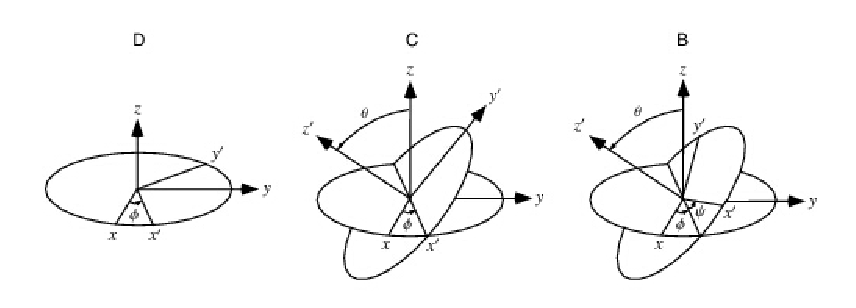
\includegraphics[width=0.96\columnwidth]{figures/euler_angles}
\caption{Demonstration of the Euler Angles. The first angle $\phi$ is with 
reapect to the $z$ axis; the second angle $\theta$ is with respect to the 
$x$ axis; the third angle $\psi$ is with repect to the $y$ axis.}
\label{fig:euler_angles}
\end{figure}

Each angle provides a rotation matrix.
\begin{equation}
D = \left(
    \begin{array}{ccc}
    \cos\phi & \sin\phi & 0 \\
    -\sin\phi & \cos\phi & 0 \\
    0 & 0 & 1 \\
    \end{array}
    \right),
C = \left(
    \begin{array}{ccc}
    1 & 0 & 0 \\
    0 & \cos\theta & \sin\theta \\
    0 & -\sin\theta & \cos\theta \\
    \end{array}
    \right),
B = \left(
    \begin{array}{ccc}
    \cos\psi & \sin\psi & 0 \\
    -\sin\psi & \cos\psi & 0 \\
    0 & 0 & 1 \\
    \end{array}
    \right)
\end{equation}
One thing that we need to keep in mind is that the order of the three 
rotations matters. Different order results in different final status. 
The composition of them $A=BCD$ is the rotation matrix
\begin{equation}
A = \left(
    \begin{array}{ccc}
    \cos\psi \cos\phi - \cos\theta \sin\phi \sin\psi & \cos\psi \sin\phi + \cos\theta \cos\phi \cos\psi & \sin\psi \sin \theta \\
    -\sin\psi \cos\phi - \cos\theta \sin\phi \cos\psi & -\sin \psi \sin\phi + \cos\theta \cos\phi \cos\psi & \cos\psi \sin\theta \\
    \sin\theta \sin\phi & -\sin\theta \cos\phi & \cos\theta \\
    \end{array}
    \right).
\label{eqn:rotation_matrix1}
\end{equation}
Angles are commonly defined according to the right hand rule. 
Namely, they have positive values when they represent a rotation that 
appears clockwise when looking in the positive direction of the axis, and 
negative values when the rotation appears counter-clockwise. 
About the ranges, $\phi$ and $\psi$ have a range of $2\pi$, and $\theta$ has 
a range of $\pi$. 



\section{Fluid Dynamics}
\label{Sec:FD}
Two most important set of governing equations that describe the motion 
of the fluid are Navier-Stokes equations and Euler equations. 
The basic method to derive both formulas is through principles of 
conservation of mass, momentum and energy
\cite{gonzalez2008continuum,lin1988mathapplied}.

\begin{itemize}
\item conservation of mass: 
\begin{equation}
\frac{\partial\rho}{\partial t}+\nabla\cdot\left(\rho\mathbf{u}\right)=0, 
\label{eqn:mass_con}
\end{equation}
where $\rho(\mathbf{x},t)$ is the spatial mass density field and 
$\mathbf{u}(\mathbf{x},t)$ is the associated spatial velocity field.
\item conservation of linear momentum:
\begin{equation}
\rho [\frac{\partial \mathbf{u}}{\partial t} + (\mathbf{u} \cdot \nabla) \mathbf{u}] = \nabla \cdot \mathbf{S} + \rho \mathbf{b}, 
\label{eqn:momentum_con}
\end{equation}
where $\mathbf{S}(\mathbf{x},t)$ is the Cauchy stress field and 
$\mathbf{b}(\mathbf{x},t)$ is the spatial body force per unit mass.
In addition, the conservation of angular momentum law leads to the 
symmetry constraint 
\begin{equation}
\mathbf{S}^{T}=\mathbf{S}.
\end{equation}
\item conservation of energy: 
\begin{equation}
\rho [\frac{\partial e}{\partial t} + (\mathbf{u} \cdot \nabla) e] = \nabla (\mathbf{S} \cdot \mathbf{u}) - \nabla \cdot \mathbf{q} + \rho r
\end{equation}
where $e(\mathbf{x},t)$ is the internal energy field per unit mass, 
$\mathbf{q}(\mathbf{x},t)$ is the Fourier-Stokes heat flux vector field, 
$r(\mathbf{x},t)$ is the heat supply field per unit mass.
\end{itemize}
Different choices of stress fields $\mathbf{S}(\mathbf{x},t)$ leads to 
equation for different type of fluid. 

\subsection*{Euler Equations}
In the world of ideal fluid which is inviscid, the Cauchy stress field is 
given as
\begin{equation}
\mathbf{S}(\mathbf{x},t) = -p(\mathbf{x},t)\mathbf{I}.
\end{equation}
Then, for the ideal fluid, in the case of absent extra body force, i.e. 
$\mathbf{b}(\mathbf{x},t) = 0$, Euler equation can be written as
\begin{eqnarray}
\left\{
\begin{aligned}
\frac{\partial \rho}{\partial t} + \nabla \cdot (\rho\mathbf{u}) &= 0 \\
\frac{\partial \mathbf{u}}{\partial t} + (\mathbf{u} \cdot \nabla) \mathbf{u} &= -\frac{1}{\rho} \nabla p \\
\frac{\partial E}{\partial t} + \nabla \cdot (\mathbf{u}(E + p)) &= 0, 
\end{aligned}
\right.
\label{eqn:Euler_eqns}
\end{eqnarray}
where $\rho$ is the fluid density, $\mathbf{u}$ is the velocity of
the fluid field, $p$ is the pressure, 
$E = \rho e + \frac{1}{2} \rho \mathbf{u}^{T} \mathbf{u}$
is the total energy density with $e$ being the specific internal
energy per unit mass. 

In order to make the system of equation closed, an equation of state is 
essential. 
Under classical ideal gas law, it can be expressed as 
\begin{equation}
p=\rho (\gamma -1) e, 
\label{eqn:equation_of_state}
\end{equation}
where $\gamma$ is the adiabatic index. 

With some algebric calculation, the momentum conservation can be 
rewritten in the conservative form 
\begin{equation}
\frac{\partial (\rho \mathbf{u})}{\partial t} + \nabla \cdot (\rho \mathbf{u} \mathbf{u}^{T} +  p\mathbf{I}) = 0,
\end{equation}
where $\mathbf{I}$ here is the $3\times3$ identity matrix.
Then, the Euler equations become a hyperbolic system when no external 
force is taken into account, 
\begin{equation}
\frac{\partial \mathbf{U}}{\partial t} + \frac{\partial \mathbf{F}(\mathbf{U})}{\partial x} + \frac{\partial \mathbf{G}(\mathbf{U})}{\partial y} + \frac{\partial \mathbf{H}(\mathbf{U})}{\partial z} = 0, 
\label{eqn:Euler_eqns_con}
\end{equation}
where 
\begin{equation}
\mathbf{U} = 
\left(
\begin{array}{c}
\rho \\ \rho u \\ \rho v \\ \rho w \\ E
\end{array}
\right),\ 
\mathbf{F} = 
\left(
\begin{array}{c}
\rho u \\ \rho u^2 + p \\ \rho u v \\ \rho u w \\ (E+p)u
\end{array}
\right),\ 
\mathbf{G} = 
\left(
\begin{array}{c}
\rho v \\ \rho u v \\ \rho v^2 + p \\ \rho v w \\ (E+p)v
\end{array}
\right),\ 
\mathbf{H} = 
\left(
\begin{array}{c}
\rho w \\ \rho u w \\ \rho v w \\ \rho w^2 + p \\ (E+p)w
\end{array}
\right)
\end{equation}

Due to the model assumption, Euler equation is most appropriate for 
simulating compressible inviscid fluid which has large Reynolds number, 
such as bullet ejection, spacecraft entrance and so on.

\subsection*{Navier-Stokes Equations}
In the incompressible Newtonian fluid case, mass density field
is uniform which means it is constant $\rho$ in the field. Thus,
\Eqn{mass_con} implies the so-called divergence-free condition 
\begin{equation}
\nabla \cdot \mathbf{u}=0.
\end{equation}
The Newtonian Cauchy stress field is given as
\begin{equation}
\mathbf{S}(\mathbf{x},t) = -p(\mathbf{x},t) \mathbf{I} + \mu (\nabla \mathbf{u}(\mathbf{x},t) + \nabla \mathbf{u} (\mathbf{x},t)^{T}), 
\end{equation}
where $\mu$ is dynamic viscosity. 

Considering only the gravitational force, i.e. 
$\mathbf{b}(\mathbf{x},t) = \mathbf{g}$, Navier-Stokes equations for 
incompressible Newtonian fluid can be rewritten as 
\begin{eqnarray}
\left\{
\begin{aligned}
\nabla \cdot \mathbf{u} &= 0 \\
\frac{\partial \mathbf{u}}{\partial t} + (\mathbf{u} \cdot \nabla) \mathbf{u} &= -\frac{1}{\rho} \nabla p + \nu \nabla^{2} \mathbf{u} + \mathbf{g}
\end{aligned}
\right.
\label{eqn:navierstoke_eqns}
\end{eqnarray}
where $\nu = \mu / \rho$ is the kinematic viscosity and $\rho_{0}$ is the 
fluid density, $\mathbf{u}$ is the velocity of the fluid field, $p$ is the
pressure. 

Due to the incompressible and viscous assumption, Navier-Stokes
equations have wide applications in physics, geoscience, aerospace and
even medical simulation when coupled with certain boundary conditions
and other appropriate constraints.



\section{Spring-Mass Model}
\label{Section:SMM}
Using spring system to model the dynamic motion of fabric surface has been
studied by computer scientists and applied mathematicians in the past several
decades, such as \cite{Choi02,Hsiao06,Ji06,Aileni10}.
Its main advantage is its simplicity and easy implementation.
We built our spring-mass model with similar idea to \cite{Choi02} and improved
it with Delingette's modification \cite{TriangularSM} to simulate the parachute
canopy.

Triangulized mesh is adopted to represent the surface where the edges of
those triangles are springs and the vertices are mass points, as shown in 
\Fig{tri_mesh}.
\begin{figure}[!ht]
    \centering
    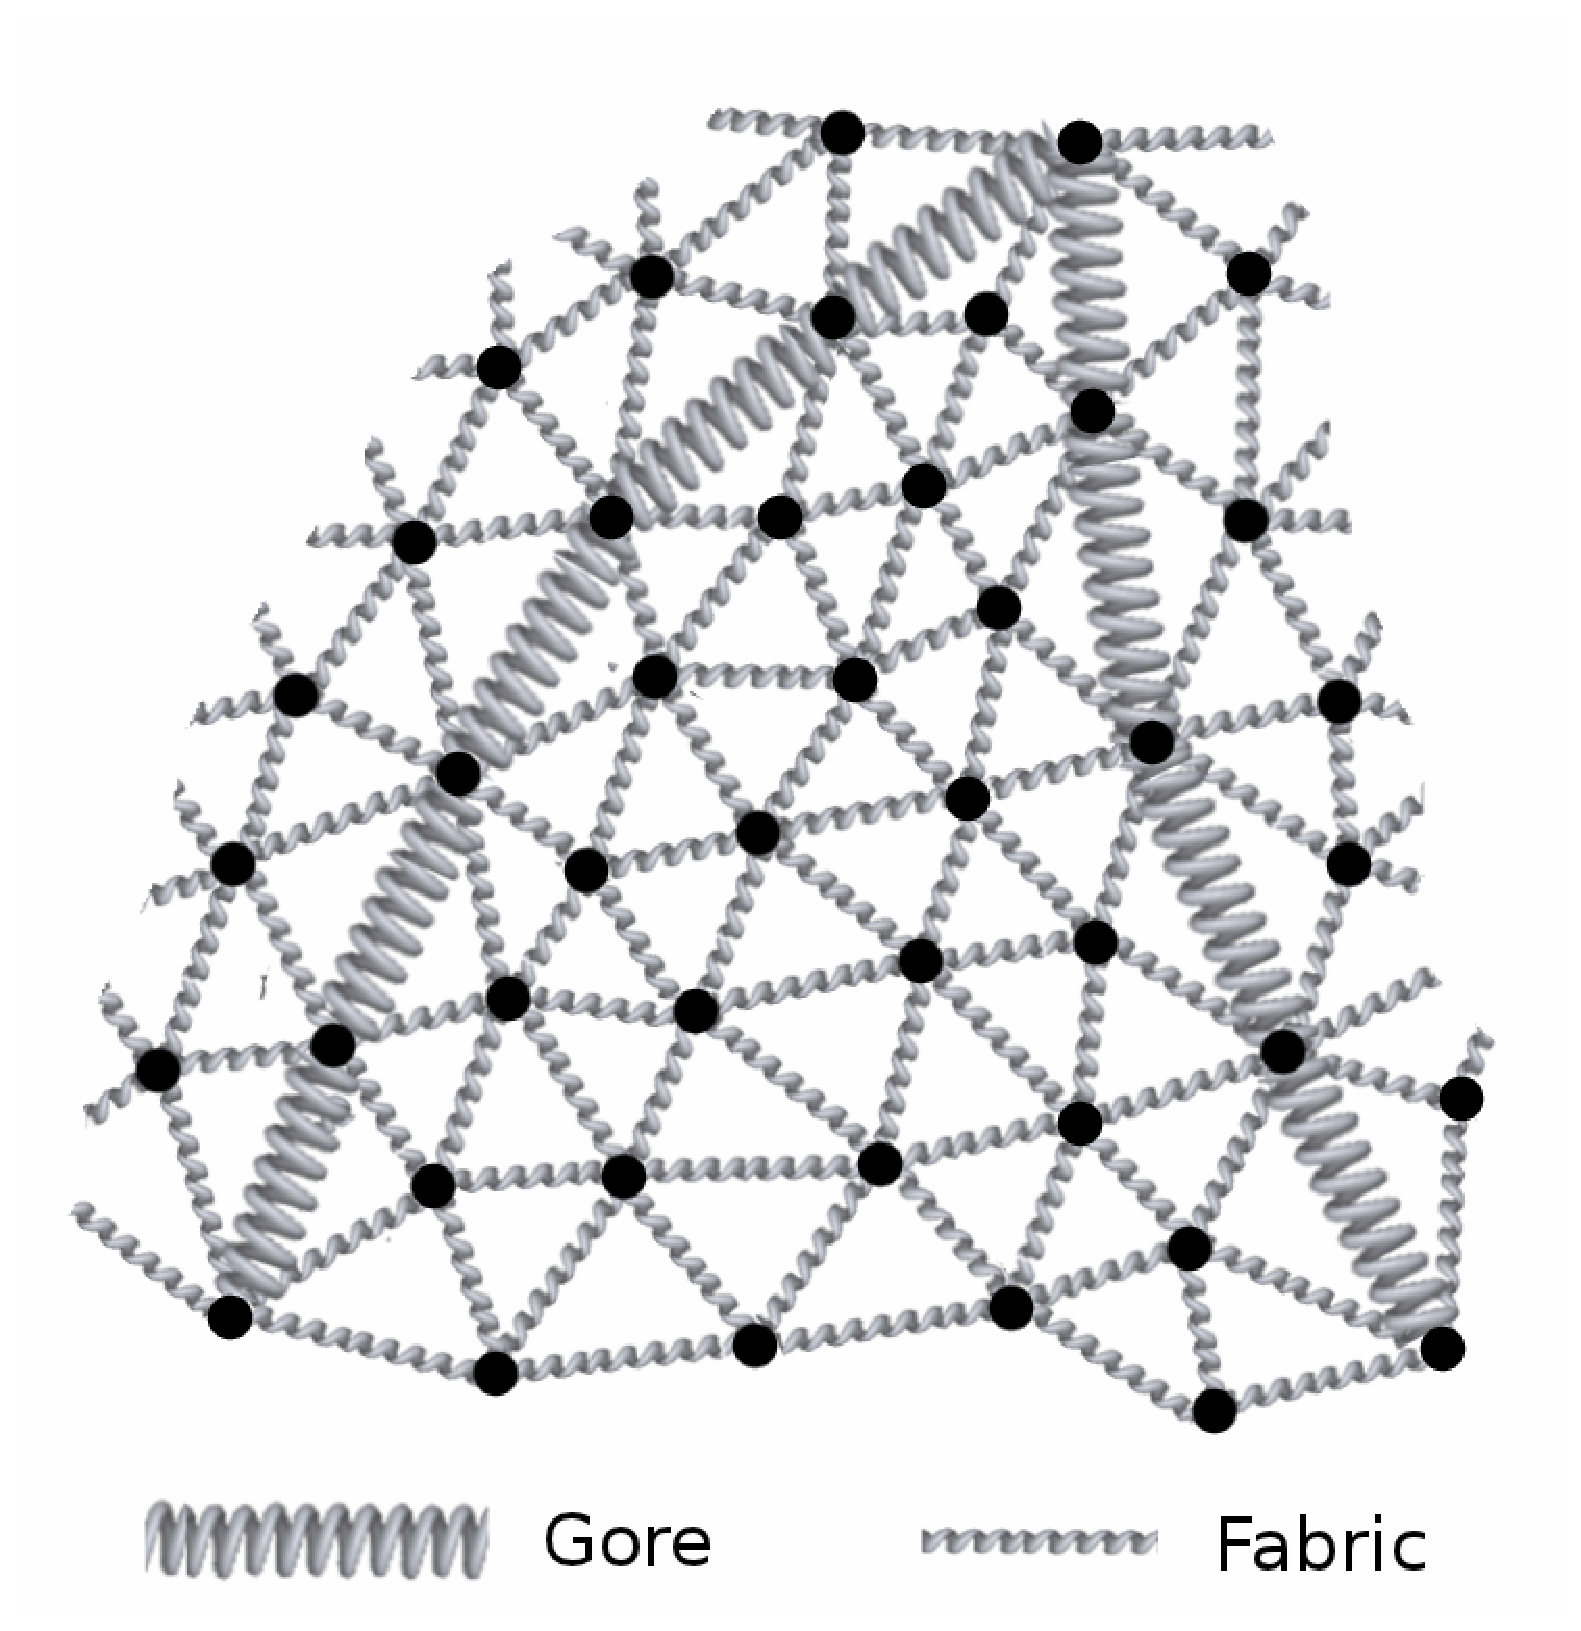
\includegraphics[width=0.6\columnwidth]{figures/goremesh}
    \caption{The spring model on a triangulated mesh. Each vertex point in
    the mesh represents a mass point with point mass $m$. Each edge of a
    triangle has a tensile stiffness. With the equilibrium lengths set during
    the initialization, the changing length of each side exerts a tensile
    spring force on the two neighboring vertex in opposite directions. Gore
    boundaries used in the parachute system can be added and modeled by curves
    with a different tensile stiffness.}
    \label{fig:tri_mesh}
\end{figure}
For each spring vertex in the spring-mass model, its motion is governed by
Newton's second law
\begin{equation}
m_{i} \frac{d\dot{\mathbf{X}}_{i}}{dt} = \mathbf{F}_i,\ i = 1,2,\cdots,N, 
\label{eqn:sm_motion}
\end{equation}
where $m_{i}$ is the mass, $\mathbf{X}_{i}$ is the position,  and
$\mathbf{F}_i$ is the total force inserted on the spring vertex.

In a elastic structure dynamics simulation, $\mathbf{F}_i$ consists of a
force $\mathbf{F}_{i}^{s}$ due to the deformation of triangles and a damping
force which slows the motion of the spring system due to friction
$\mathbf{F}_{i}^{d}$.
The external force $\mathbf{F}_{i}^{e}$, representing the effects of air drag
and gravity is considered by adding an additional term on the right-hand side.

Our spring-mass model \cite{LiChernKimLi12,shi2015verification} assumes the
force to stretch the spring is proportional to its displacement from the
equiblibrium distance between the two adjacent spring vertices.
In addition, the force that prevents the change of angles is described by the
angular stiffness in Delingette's modification \cite{TriangularSM} which is
favored by its relation to the elastic spring model in continuum mechanics.
\begin{figure}
\centering
\begin{subfigure}{0.48\columnwidth}
    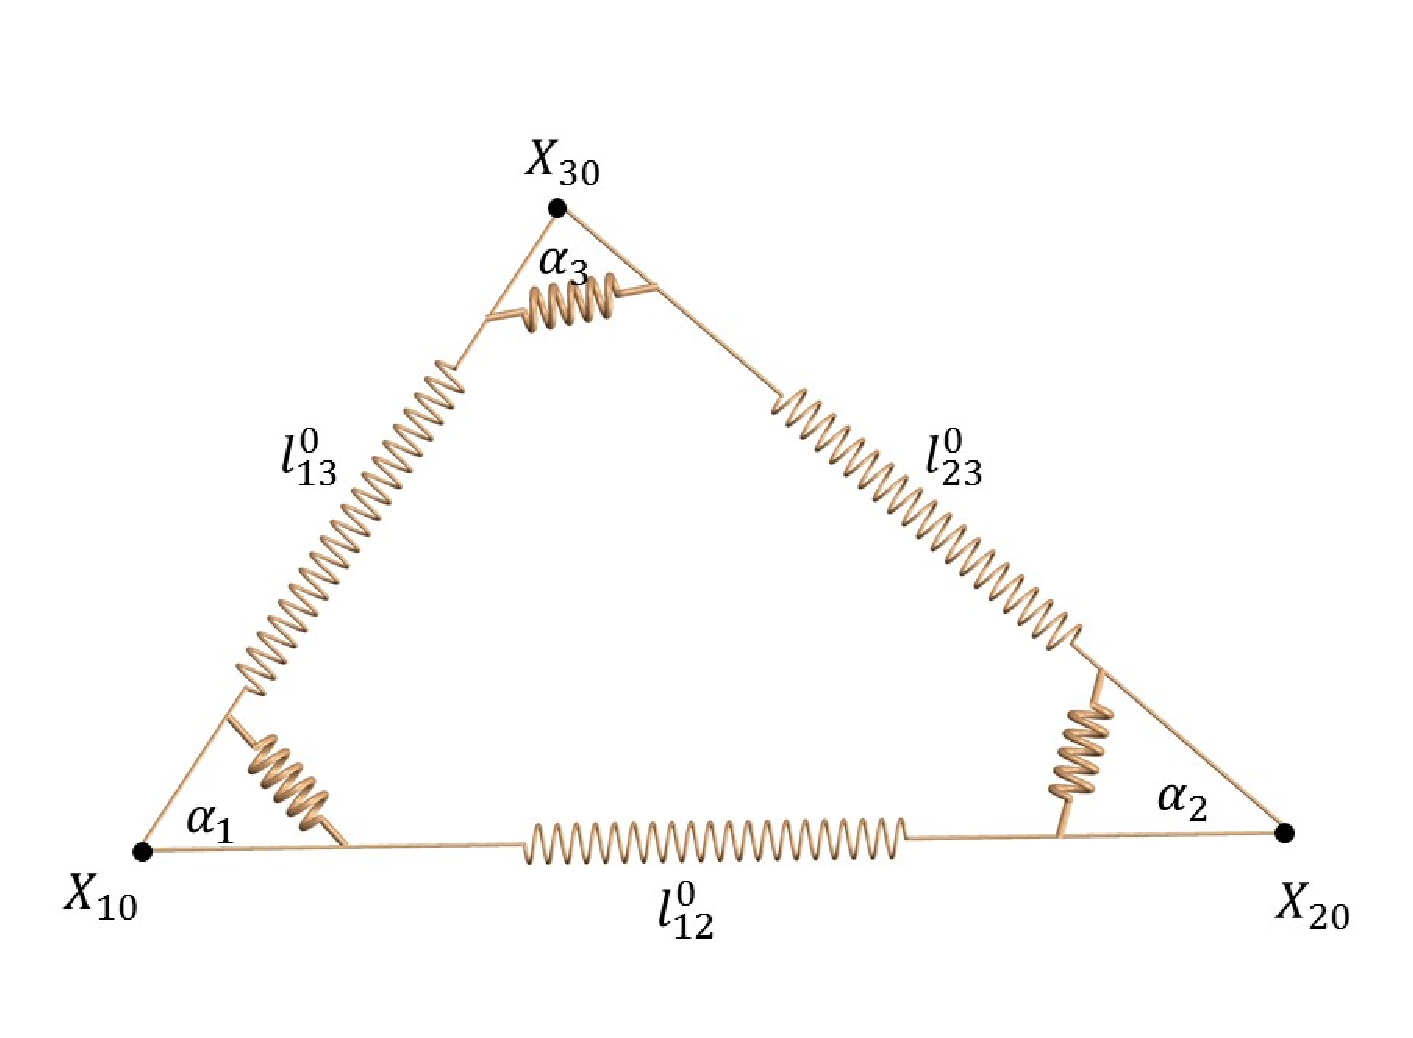
\includegraphics[width=1.0\textwidth]{figures/rest}
    \caption{Triangle in the rest status}
\end{subfigure}
\begin{subfigure}{0.48\columnwidth}
    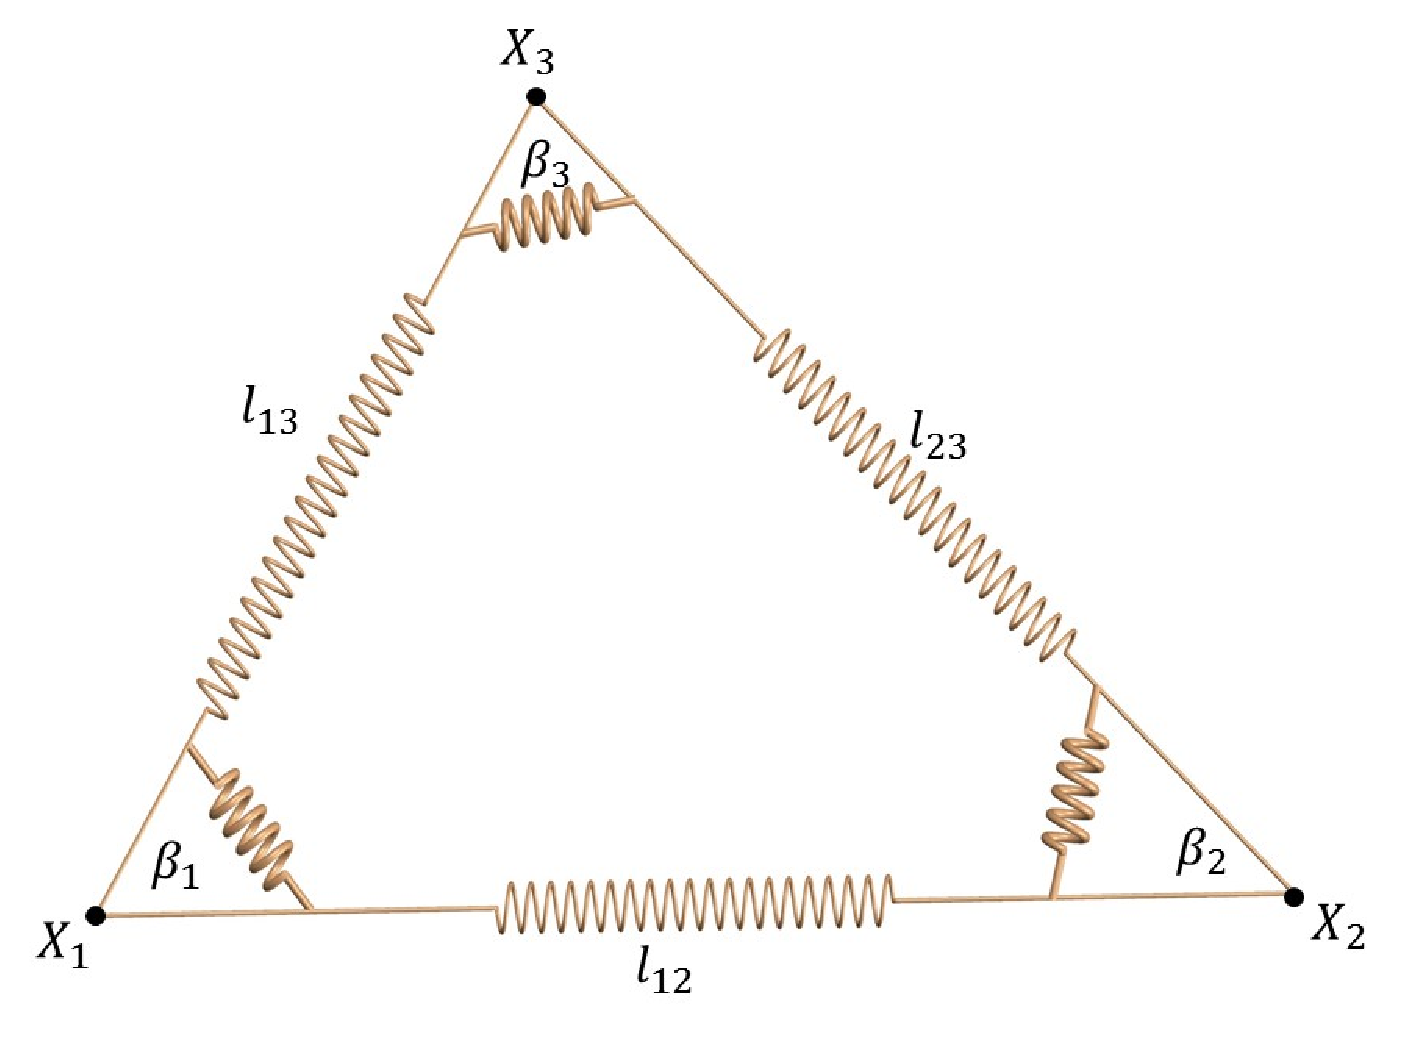
\includegraphics[width=1.0\textwidth]{figures/deformed}
    \caption{Triangle in the deformed status}
\end{subfigure}
\caption{Left: rest triangle $T_{X_0}$ with vertex $X_{i0}$. Right:
deformed triangle $T_{X}$ with vertex $X_{i}$. Each edge is represented as
a spring and the tensile stiffness prevents the deformation of the edge.
At each corner, an artifical spring prevents the change of angles.}
\label{fig:rest_deformed_tri}
\end{figure}

With $dl_{ij} = l_{ij} - l_{ij}^0$ representing the length change of the
spring between $\mathbf{X}_{i}$ and $\mathbf{X}_{j}$, the potential energy
is given in \cite{TriangularSM} as
\begin{equation}
W(T) = \sum_{\substack{i=1\\j=(i+1) \mod 3}}^{3}\frac{1}{2}k_{ij}^{T}(dl_{ij})^{2} + \sum_{\substack{i=1\\j=(i+1) \mod 3\\k=(i+2) \mod 3}}^{3}\gamma_{i}^{T}dl_{ij}dl_{ik}, 
\label{eqn:sm_energy}
\end{equation}
where the first term is the stretching energy, and the second term is the
angular energy from Delingette's modification.

In \Eqn{sm_energy}, the tensile stiffness and the angular stiffness are
calculated as
\begin{equation}
k_{ij}^{T} = \frac{(l_{ij}^0)^2 (2\cot^2\alpha_k(\lambda+\mu)+\mu)}{8A}, 
\label{eqn:t_stiffness}
\end{equation}
\begin{equation}
\gamma_{i}^{T} = \frac{l_{ik}^0 l_{ij}^0 (2 \cot\alpha_j \cot\alpha_k (\lambda+\mu) - \mu)}{8A},
\label{eqn:a_stiffness}
\end{equation}
where $A$ denotes the area of the triangle in equilibrium, $i = 1,2,3$,
$j = (i+1)\ \mod\ 3$, and $k = (i+2)\ \mod\ 3$.
$\lambda$ and $\mu$ are the Lam\'{e} coefficients of the material, and they
are related to Young's modulus $E$ and the Poisson ratio $\nu$ \cite{Gere2004}
\begin{equation}
\lambda=\frac{E\nu}{1-\nu^2},\ \mu=\frac{E(1-\nu)}{1-\nu^2}.
\label{eqn:Lame_coeff}
\end{equation}

Apply Rayleigh-Ritz analysis and it tells that the fabric surface, represented
by the triangular mesh, should evolve by minimizing its membrane energy.
Therefore, along the opposite derivative of that energy with respect to the
nodes of the system, that is, the deformed positions $X_i$:
\begin{align}
\mathbf{F}_{i}^{s}(T_{\mathbf{X}_{0}}) &=  -\frac{\partial W(T_{\mathbf{X}_{0}})}{\partial \mathbf{X}_{i}} \notag \\
&= \sum_{\substack{j=1\\j\neq i}}^{3} k_{ij}^{T_{\mathbf{X}_{0}}} dl_{ij} \frac{\mathbf{X}_{j}-\mathbf{X}_{i}}{l_{ij}} + 
\sum_{\substack{j=1,j\neq i\\k\neq i,k\neq j}}^{3} (\gamma_{k}^{T_{\mathbf{X}_{0}}} dl_{kj} + \gamma_{i}^{T_{\mathbf{X}_{0}}}dl_{ij}) \frac{\mathbf{X}_{k}-\mathbf{X}_{i}}{l_{ik}}
\label{eqn:tri_sm_force}
\end{align}
This is the force on vertex $\mathbf{X}_{i}$ due to the deformation of the
triangular $T_{\mathbf{X}_{0}}$ and it can be split into two components
\begin{equation}
\mathbf{F}_{i}^{s}(T_{\mathbf{X}_{0}}) = \mathbf{F}_{ij}^{s}(T_{\mathbf{X}_{0}}) + \mathbf{F}_{ik}^{s}(T_{\mathbf{X}_{0}}),
\end{equation}
where $j=(i+1)\ mod\ 3$ and $k=(i+2)\ mod\ 3$, and
\begin{align}
\mathbf{F}_{ij}^{s}(T_{\mathbf{X}_{0}}) &= k_{ij}^{T_{\mathbf{X}_{0}}} dl_{ij} \mathbf{e}_{ij} + (\gamma_i^{T_{\mathbf{X}_{0}}} dl_{ik} + \gamma_{j}^{T_{\mathbf{X}_{0}}} dl_{jk}) \mathbf{e}_{ij}, \\
\mathbf{F}_{ik}^{s}(T_{\mathbf{X}_{0}}) &= k_{ik}^{T_{\mathbf{X}_{0}}} dl_{ik} \mathbf{e}_{ik} + (\gamma_i^{T_{\mathbf{X}_{0}}} dl_{ij} + \gamma_{k}^{T_{\mathbf{X}_{0}}} dl_{kj}) \mathbf{e}_{ik}.
\end{align}
\begin{figure}[!ht]
    \centering
    \includegraphics[width=0.4\columnwidth]{figures/force_ij}
    \caption{Two triangles $T_1$ and $T_2$ share $\mathbf{X}_i$ and
    $\mathbf{X}_j$; the other vertex of triangles $T_1$ and $T_2$ are
    $\mathbf{X}_m$ and $\mathbf{X}_n$ respectively.}
    \label{fig:force_ij}
\end{figure}

Since each edge is shared by two triangles, the spring force between two vertex
$\mathbf{X}_i$ and $\mathbf{X}_j$, as shown in \Fig{force_ij}, is the
summation of the effects from both triangles and has
the following formula:
\begin{align}
\mathbf{F}_{ij}^{s} &= \mathbf{F}_{ij}^{s}(T_1) + \mathbf{F}_{ij}^{s}(T_2) \notag \\
&= [(k_{ij}^{T_1} + k_{ij}^{T_2})dl_{ij} + (\gamma_{i}^{T_1}dl_{im} + \gamma_{j}^{T_1}dl_{jm} + \gamma_{i}^{T_2}dl_{in} + \gamma_{j}^{T_2}dl_{jn})]\mathbf{e}_{ij} \notag \\ 
&= \tilde{k}_{ij}dl_{ij}\mathbf{e}_{ij} + \tilde{\gamma}_{ij}dl_{ij}\mathbf{e}_{ij},
\label{eqn:sm_force_new}
\end{align}
where $\tilde{k}_{ij} = k_{ij}^{T_1}+k_{ij}^{T_2}$, $\tilde{\gamma}_{ij} = 
(\gamma_{i}^{T_1}dl_{im} + \gamma_{j}^{T_1}dl_{jm} + \gamma_{i}^{T_2}dl_{in} + 
\gamma_{j}^{T_2}dl_{jn})/dl_{ij}$.

As mentioned earlier, a damping force slows the spring system and we take it
into account with the formula
\begin{equation}
\mathbf{F}_{i}^{d} = c \mathbf{V}_{i}^{(int)},
\label{eqn:damp_force}
\end{equation}
where $c$ is the viscous damping coefficient and $\mathbf{V}_{i}^{(int)}$ is
the internal component of the vertex velocity that is due to the spring force
only.
On the other hand, the external component $\mathbf{V}_{i}^{(ext)}$ involves
effects from gravity, fluid, and so on.
With all forces considered, the equation of motion (\ref{eqn:sm_motion}) can
be re-written as an ODE system
\begin{equation}
\left\{
\begin{aligned}
\dot{\mathbf{X}}_{i} &= \mathbf{V}_{i} \\
m_{i} \dot{\mathbf{V}}_{i} &= \mathbf{F}_{i}^{s} + \mathbf{F}_{i}^{d} + \mathbf{F}_{i}^{e}
\end{aligned}
\right.
\label{eqn:sm_ODEs}
\end{equation}
where $\mathbf{V}_{i}$ is the total velocity, i.e. the summation of
$\mathbf{V}_{i}^{(int)}$ and $\mathbf{V}_{i}^{(ext)}$.

One thing that we need to keep in mind is that the canopy-like structures
are lack of bending stiffness, therefore, the bending force can be negligible
in the simulation of the parachute system.
However, for simulations of other kind of fabric structures, bending force
can be taken into account by adding an artificial spring between the two
vertex, $\mathbf{X}_{m}$ and $\mathbf{X}_{n}$, that are not shared by two 
adjacent triangles.
This additional resistance prevents local clustering of triangle meshes.



\section{Parachutist/Cargo Inclusion}
\label{PCI}
The dimensions of parachutist or cargo are usually smaller than the parachute
canopy surface.
However, when the fluid flow across the parachutist or cargo, the dynamical
behavior of the flow will have different patterns based on different Reynolds
numbers.
These turbulent flow will reach the parachute canopy surface later and
contribute to the motion of the canopy surface.
Therefore the inclusion of parachutists will make numerical simulation of
parachute systems much closer to reality.
\Fig{cargo_amplification} show three examples of connecting the suspension 
lines to the parachutist.
\begin{figure}
\centering
\begin{subfigure}{0.32\columnwidth}
    \includegraphics[width=1.0\textwidth]{figures/box}
    \caption{A cuboid cargo}
\end{subfigure}
\begin{subfigure}{0.32\columnwidth}
    \includegraphics[width=1.0\textwidth]{figures/ball}
    \caption{A spherical cargo}
\end{subfigure}
\begin{subfigure}{0.32\columnwidth}
    \includegraphics[width=1.0\textwidth]{figures/human}
    \caption{Human parachutist}
\end{subfigure}
\caption{Three examples of the connection amplification between the 
suspension lines and different types of cargos. Besides these three, 
\FronTierp is capable of generating different kinds of rigid bodies.}
\label{fig:cargo_amplification}
\end{figure}

In our model, the parachutist can be either a mass point with no instance or
a rigid body with finite volume.
In the former case, no interaction between the parachutist and the fluid is
considered.
Therefore, no turbulent flow is observed between the space of the canopy
surface and the parachutist.
However, in the latter case, the fluid-structure interaction is non-negligible,
and there are two important aspects need to be taken into account carefully.
\begin{itemize}
\item Calculation of force and torque on the cargo. \\
    The force consists of three parts: force of gravity, force exerted by the
    fluid flow and force from the suspension lines.
    The force and corresponding torque are then applied to the parachutist for
    translation and rotation.
    \begin{itemize}
    \item The force exerted by the fluid flow can be broken into two parts:
    force due to pressure difference and force due to friction (viscosity).
    In the parachute simulation, we consider the first part as the dominant
    component.
    \begin{eqnarray}
    \begin{aligned}
    F_p &= \int_{s} (p - p_0)\hat{n} dA, \\
    \end{aligned}
    \end{eqnarray}
    where $\hat{n}$ is the normal direction to the surface with area $dA$,
    $p_0$ is the pressure far away from the surface $dA$
    and $p$ is the pressure at surface $dA$.
    \end{itemize}
\item Propagation of the rigid body. \\
    The propagation must maintain the geometric shape of the parachutist.
    This has perfect match with the Lagrangian propagation of the front
    tracking method in \FronTierp \cite{GliGroLi99a,DuFixGli05}.
    \begin{itemize}
    \item The translational motion is trivial.
    Simply apply the acceleration caused by the total force to the center of
    mass, and correspondingly propagate each point of the parachutist.
    \item The rotational motion with respect to the center of mass is governed
    by Euler's equations \Eqn{eulers_equation2} of rigid body dynamics
    \cite{goldstein2001}.
    \end{itemize}
\end{itemize}



\section{Collision Handling}
\label{Sec:CH}
In cloth simulations, it is almost impossible to totally avoid collision. 
Thus, robust collision detection and handling is very important to make the 
numerical simulation visually realistic. 
The collision detection and handling problem has attracted scientists in 
many fields. 
Early work by Terzopoulosi \emph{et al.}, \cite{terzopoulos1987elastically, 
terzopoulos1988modeling, terzopoulos1991deformable}, is governed 
by the mechanical laws of continuous bodies. 
Since then, many well-performed and well-known techniques are proposed by 
different groups, like Carignan \emph{et al.} \cite{carignan1992dressing}, 
Volino \emph{et al.} \cite{volino1995collision, volino1995versatile, 	volino1996evolving}, Baraff \emph{et al.} \cite{baraff1998large, 
baraff2003untangling}, Bridson \emph{et al.} \cite{Bridson2002collsn} and 
so on.  
Our collision algorithm is mainly based on the idea of combining a fail-safe 
geometric collision method and the repulsion force method that is presented 
in \cite{Bridson2002collsn}. 
In addition, we extended this algorithm to make it work for not only cloth, 
but also strings and rigid bodies.

In \Fig{collsn_demo}, the process of the collision algorithm is 
demonstrated for collision between fabric structure and a static object. 
As for self-collision of the fabric structure and collision between fabric 
structure and a movable object, the handling is similar. 
The only difference lies in how they move back to the time right before 
collision and how the impulse is applied.
\begin{figure}[!ht]
    \centering
    \begin{subfigure}{0.48\columnwidth}
	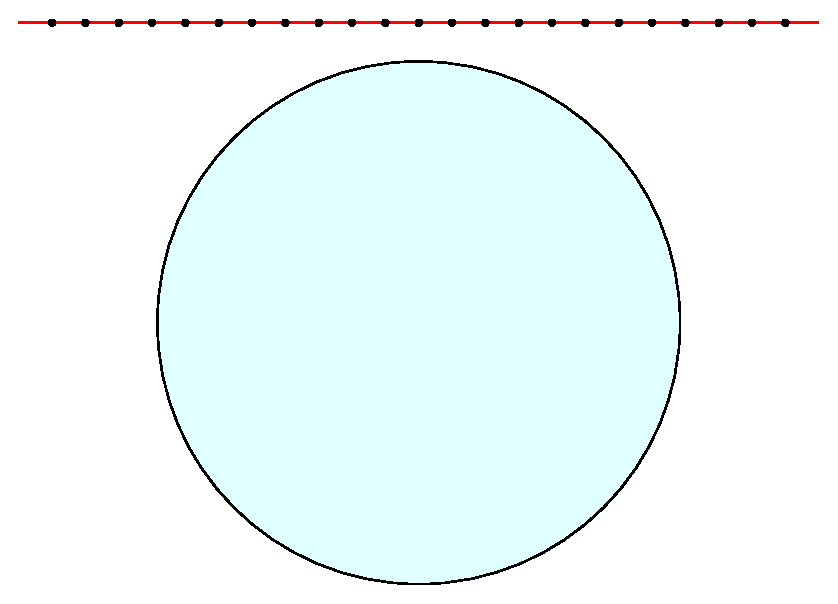
\includegraphics[width=\textwidth]{figures/collsn_demo_0}
	\caption{before collision}
    \end{subfigure}
    \begin{subfigure}{0.48\columnwidth}
	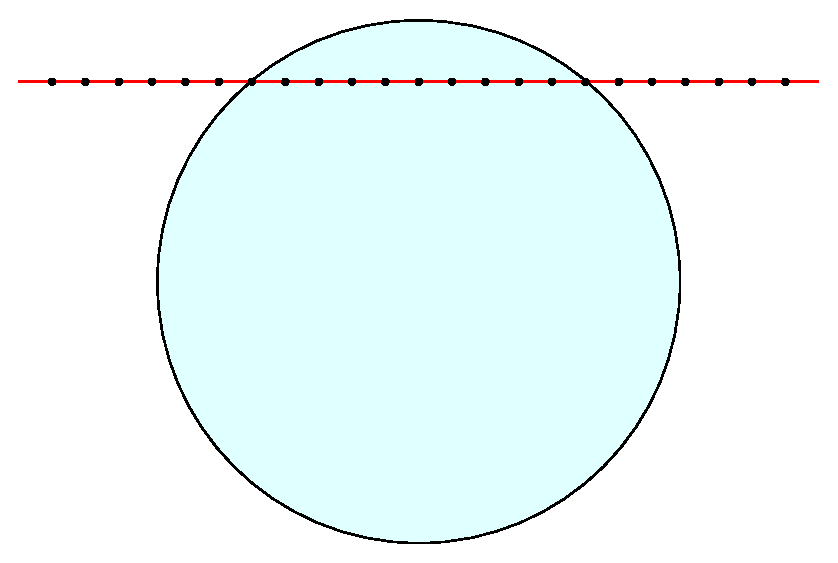
\includegraphics[width=\textwidth]{figures/collsn_demo_1}
	\caption{collision occurs}
    \end{subfigure} \\
    \begin{subfigure}{0.48\columnwidth}
	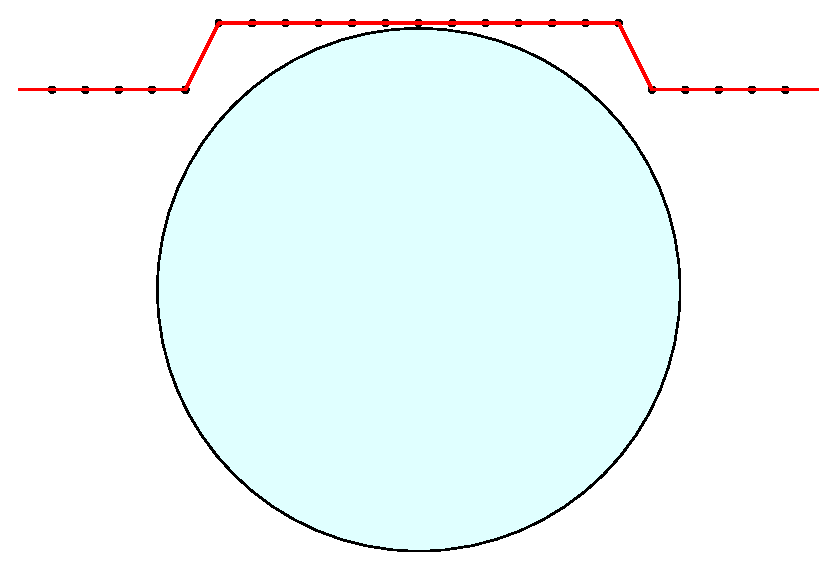
\includegraphics[width=\textwidth]{figures/collsn_demo_2}
	\caption{move back}
    \end{subfigure}
    \begin{subfigure}{0.48\columnwidth}
	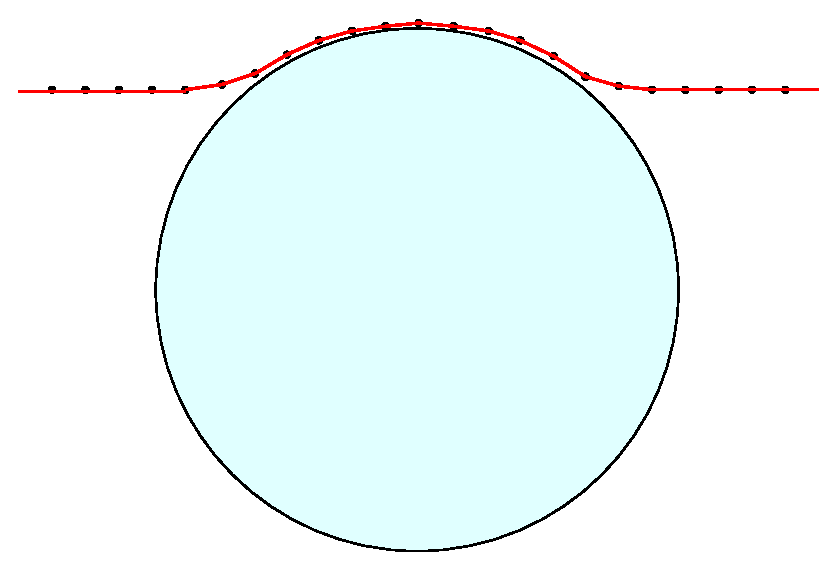
\includegraphics[width=\textwidth]{figures/collsn_demo_3}
	\caption{apply impulse}
    \end{subfigure}
    \caption{A demonstration of process how to resolve the collision. The red 
    line represents the fabric structure; the light-blue disk represents an 
    object; the points on the red line are the mass points in the spring 
    model.}
    \label{fig:collsn_demo}
\end{figure}

The following is a summary of the collision algorithm. The detection is
done by axis-aligned bounding box (AABB) tree, and the details of impulse
and impact zone technique are discussed in the following chapter.
\begin{itemize}
\item Pre-processing:
    \begin{itemize}
    \item Starting at $t^n$ with a time step $\Delta t$, record
    current positions $\mathbf{x}^{n}$ and velocities $\mathbf{v}^{n}$.
    \item Propagate all structures to the candidate positions
    $\mathbf{x}^{can}$ with candidate velocities
    $\mathbf{v}^{can}$ at time $t^{n+1}$, and compute the average velocity
    during this time step,
    $\mathbf{v}^{ave} = (\mathbf{x}^{can} - \mathbf{x}^{n}) / \Delta t$.
    \item Connect points on each rigid body (static or movable) as one
    impact zone.
    \end{itemize}
\item Detection and Handling:
    \begin{itemize}
    \item Perform the proximity check for $\mathbf{x}^{n}$ and apply
    impulse and friction to update $\mathbf{v}^{ave}$.
    \item Perform the collision check for propagation from $\mathbf{x}^{n}$
    with velocity $\mathbf{v}^{ave}$, and resolve collisions by applying
    impulse and rigid impact zones technique to update $\mathbf{v}^{ave}$.
    \item Update the candidate position of all the points by
    $\mathbf{x}^{can} = \mathbf{x}^{n} + \Delta t \mathbf{v}^{ave}$.
    \item If there is no more collision with respect to $\mathbf{x}^{can}$,
    continue to the post-processing; otherwise, repeat the detection and
    handling process.
    \end{itemize}
\item Post-processing:
    \begin{itemize}
    \item Advance the $\mathbf{v}^{ave}$ to $\mathbf{v}^{can}$ for points
    involved in collision, and, meanwhile, update the center of mass and
    center of mass velocity of the movable rigid bodies.
    \item Continue to the next time step with
    $\mathbf{x}^{n+1} = \mathbf{x}^{can}$ and
    $\mathbf{v}^{n+1} = \mathbf{v}^{can}$ for all points.
    \end{itemize}
\end{itemize}



\newpage
